\iffalse \bibliography{include/backmatter/magnus,include/backmatter/philip} \fi
\chapter{Related Work}
In this section we introduce (1) the process of identifying current literature and (2) outline current research on the performance overhead of utilising Docker.

\section{Gathering Related Work}
The snowballing search approach for systematic literature studies is used to find relevant literature on the topic of this paper. The snowballing approach is the process of using the reference list or citations of a paper in order to identify additional papers. The guidelines for conducting a snowballing search approach, presented by Wohlin \cite{Wohlin}, are followed. 

\subsection{Start Set}
In order to begin the snowballing search approach, a collection of papers are required. In order to identify a start set of papers, keywords are extracted from the research questions, taking synonyms into account. Formulating a search-string from keywords that are broad and cover multiple areas of research may result in collecting a vast amount of literature. For that reason, broad keywords are broken down into more specific and detailed keywords specific to this study. The resulting search string used for a provisional start-set is found in table~\ref{search-string}. \\

The search string was applied to the Scopus \cite{scopus} database which resulted in finding 298 papers. The documents were then limited by subject area resulting in 215 papers. A screening process was then applied to the provisional start-set. The screen process included reading the title and if necessary the abstract to determine if the paper is relevant to this study. 

\begin{table}[h]
\centering
\begin{tabular}{p{15cm}}
TITLE-ABS-KEY(Performance OR Comparison OR Latency OR Evaluation OR Container-Based OR Linux Containers OR Lightweight Virtualization OR Container Cloud OR Docker) AND ( LIMIT-TO(SUBJAREA,"COMP" ) )
\end{tabular}
\caption{Search String}
\label{search-string}
\end{table}



%-------------------------------------------------------------------%
%Minimizing latency of real-time container cloud for software radio access networks
%Internet of Things gateways meet linux containers: Performance evaluation and discussion
%KVM, Xen and Docker: A performance analysis for ARM based NFV and cloud computing
%Hypervisors vs. Lightweight Virtualization: a Performance Comparison
%A performance isolation analysis of disk-intensive workloads on container-based clouds

%Accelerating Regression Testing for Scaled Self-Driving Cars with Lightweight Virtualization-A Case Study  **
%An updated performance comparison of virtual machines and Linux containers **
%Performance evaluation of containers for HPC **
%A Container-based Elastic Cloud Architecture for Real-Time Full-Motion Video (FMV) Target Tracking **

%Performance comparison and tuning of virtual machines for sequence alignment software  (Article) *** some performance results

%ocker reference
%http://ieeexplore.ieee.org/stamp/stamp.jsp?tp=&arnumber=7036275
%-------------------------------------------------------------------%




%Start Set: 
%In order find papers, we applied the following technique. 

%Constructing Search String: In order to formulate a search string, major terms were derived from the research questions. For these major terms, alternative spelling and snynonyms were included. 

%Resources to be Searched: Scopus

%Search Constraints: We will search all papers related to the research questions and applied no search constrainsts.


%Backward Snowballing: 

%orwards Snowballing: 

%Inclusion and Exclusion: 

%-> Resulting x ammount of papers. 

%Then we being the related work section. 



%This section uses some of the processes from a systematic mapping study (http://www.bcs.org/upload/pdf/ewic_ea08_paper8.pdf)

%Snowballing is used to prepare related work. 

%First step is to set up a search string. The search string is derived from the research questions, but with more detail. 

%The search string is as follows: \textit{TITLE-ABS-KEY(Performance OR Comparison OR Latency OR Evaluation OR Container-Based OR Linux Containers OR Lightweight Virtualization OR Container Cloud OR Docker )}

%The search string was applied to Scopus database. It retrieved 298 documents. 

%Screening was then done on the 298 papers where relevant papers were extracted 

%Keywording abstracts was then applied 

%Since the author of \cite{Wohlin} states there is no silver bullet for identifying a good start set, steps from the systematic mapping process \cite{Petersen} are used. 
 
%\begin{figure}[ht]
%\centering
%     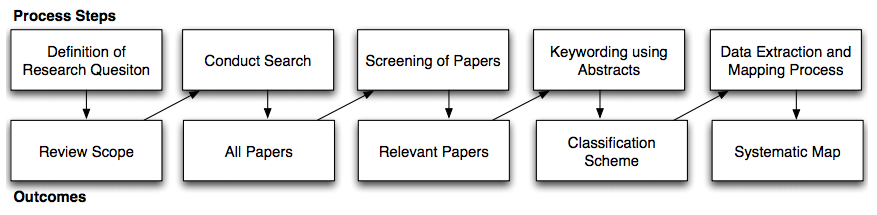
\includegraphics[width=1.0\textwidth]{./figure/sms.png}
%      \caption{The Systematic Mapping Process \cite{Petersen}}
%       \label{mapping-study}
%\end{figure}


\subsection{Iterations}

We then applied techniques from snowballing, to go forward and backwards 


